\documentclass[a4paper]{report}
\usepackage{anysize}
\marginsize{3cm}{3cm}{2cm}{2cm}
\usepackage[utf8]{inputenc}
\usepackage[T1]{fontenc}
\usepackage{textcomp}
\usepackage[french]{babel}
\usepackage{graphicx}
\usepackage{float}
\usepackage{mathtools}
\usepackage{listings}
\usepackage{listingsutf8}
\graphicspath{ {img/} }
\setcounter{secnumdepth}{4}
\setcounter{tocdepth}{2}

% addresse du tuto pour activer la coloration du code
% http://blog.hikoweb.net/index.php?post/2012/02/04/Colorer-du-code-source-dans-un-rapport-LaTeX-avec-Minted
\usepackage{minted}

\newcommand{\english}[1]{\textit{#1}}
\newcommand{\brand}[1]{\textbf{#1}}
\newcommand{\nexys} {Nexys3}
\newcommand{\fpga} {FPGA}
\newcommand{\fpgas} {FPGAs}
\newcommand{\TODO}[1]{\textbf{\textcolor{blue}{#1}}}

\usepackage{hyperref}
\hypersetup{
    bookmarks=true,         % show bookmarks bar?
    unicode=false,          % non-Latin characters in Acrobat’s bookmarks
    pdfnewwindow=true,      % links in new window
    colorlinks=true,       % false: boxed links; true: colored links
    linkcolor=black,        % color of internal links (change box color with linkbordercolor)
    citecolor=magenta,        % color of links to bibliography
    filecolor=magenta,      % color of file links
    urlcolor=[rgb]{0,0,0.5}           % color of external links
}

\definecolor{mygreen}{rgb}{0,0.6,0}

\usepackage{color}
\lstset{
  numbers=none,
  frame=single,
  tabsize=4,
  breaklines=true,
  keywordstyle=\color{blue}\textbf,
  commentstyle=\color{mygreen}\textit,
  stringstyle=\color{red},
  basicstyle=\footnotesize,
  backgroundcolor=\color{white}
}

% Pieds de page et en-tête
\usepackage{fancyhdr}
\pagestyle{fancy}
\lhead{}
\chead{}
\rhead{}
\renewcommand{\headrulewidth}{0pt}
\renewcommand{\footrulewidth}{0.4pt}
\lfoot{Projet Systèmes Informatiques : du compilateur vers le microprocesseur}
\cfoot{}
\rfoot{Page \thepage}


\begin{document}

\begin{titlepage}

\centering

{\Large {\bf Rapport de projet}}\\

\vspace{30pt}

{\huge Architectures matérielles de systèmes informatiques}\\
\vspace{50pt}
{\Huge Du compilateur vers le microprocesseur}\\

\vspace{130pt}

\underline{Chargé de TP :} \\
\vspace{5pt}
Fernand LONE-SANG

\vspace{30pt}
Benoît GAYRAUD\\
Matthieu LONGO

\vspace{5pt}

\par
{\tt bgayrau@etud.insa-toulouse.fr}\\
{\tt longo@etud.insa-toulouse.fr}\\

\vspace{20pt}

\vfill {\bf Description}\medskip \\
  \fbox{
    \begin{minipage}{0.9\textwidth}
      Conception d'un microprocesseur de type RISC avec un pipeline à 5 étages.\\
      Développer un compilateur en utilisant LEX et YACC en utilisant les concepts abordés en cours d'Automates \& Langages.
    \end{minipage} 
  }

\vspace{50px}


\begin{center}
DGEI\\
4\up{ème} année  Informatique et Réseaux\\
2012-2013
\end{center}
\begin{figure}[!h]
    \centering
    
\includegraphics[scale=0.45]{logoINSA.jpg}
\end{figure}


\begin{center}
\LaTeX
\end{center}

\end{titlepage}


\tableofcontents

\newpage

\chapter*{Introduction} \addcontentsline{toc}{chapter}{Introduction}
Le projet s'est articulé en deux axes, le premier autour de la conception d'un microprocesseur de type RISC avec pipeline, le deuxième autour du développement d'un compilateur en utilisant les logiciels LEX et YACC. L'objectif était de réaliser un système informatique complet.\\
Dans un premier temps, nous parlerons de l'architecture matérielle du microprocesseur que nous avons implémenté sur la \nexys{}, une carte de chez Xilinx possédant un FPGA Spartan6. Au cours de cette partie, nous aborderons les spécificités de notre architecture.\\
Par la suite, nous présenterons les éléments du langage C supportés par le compilateur, le fonctionnement des deux sous-modules dont il est composé et les fichiers intermédiaires générés.



\newpage


\chapter{Développement du microprocesseur}

Après avoir regardé les spécifications du microprocesseur, nous l'avons implémenté en deux temps.\\
Premièrement, nous avons implémenté les sous-modules du processeur(ALU, banc de registres) et ceux extérieurs au processeur comme la RAM et la ROM. Nous avons pu effectuer des testbenchs sur chacun des composants afin de vérifier son bon fonctionnement. Il a fallu  également synthétiser les modules pour vérifier qu'ils étaient bien implémentables.\\
Par la suite, par soucis de simplicité, nous avons intégrer tous ces modules dans un macro-module. Nous avons donc à la fois la RAM et l'ALU dans le même module alors que sur un vrai processeur, cela ne devrait jamais se produire. C'est au cours de cette deuxième étape que l'on a eu à introduire les unités de saut et de gestion du pipeline.\\
Enfin, on suivra l'exécution d'un programme de test sur un chronogramme et on concluera sur les points à améliorer ou à implémenter par rapport aux spécifications.

\newpage

\section{Les spécifications}
Nous avions principalement deux points à respecter : le jeu d'instructions et la présence d'un pipeline à 5 niveaux.

\subsection{Le jeu d’instructions}

Le jeu d'instructions proposé est orienté registre. La présence de \texttt{LOAD} et \texttt{STORE} indique qu'il s'agit d'un processeur RISC LOAD/STORE. Les intructions sont de taille fixe, toutes codées sur 32 bits sous le format suivant : \textbf{A  CodeOP  B  C} (8 bits pour A, 8 bits pour le code opération, 8 bits pour B et 8 bits pour C). Nous n'utiliseront pas forcément tous les octets pour coder une instruction. Pour certaines opérations simples comme le saut inconditionnel, 2 octets suffiront et les 2 restants constitueront du \textit{padding}. La figure \ref{tab:instructions-proc} détaille le jeu d'instruction du processeur.

\begin{table}[h!]
  \centering
  \begin{tabular}{| l | l | l | l |}
    \hline
    Addition & \texttt{0x01} & \texttt{ADD  R$_{X}$  R$_{Y}$  R$_{Z}$} & \texttt{R$_{X}$ $\leftarrow$ R$_{Y}$ $+$ R$_{Z}$} \\ \hline
    Soustraction & \texttt{0x03} & \texttt{SUB  R$_{X}$  R$_{Y}$  R$_{Z}$} & \texttt{R$_{X}$ $\leftarrow$ R$_{Y}$ $-$ R$_{Z}$} \\ \hline
    Multiplication & \texttt{0x02} & \texttt{MUL  R$_{X}$  R$_{Y}$  R$_{Z}$} & \texttt{R$_{X}$ $\leftarrow$ R$_{Y}$ $*$ R$_{Z}$} \\ \hline
    Division (non gérée) & \texttt{0x04} & \texttt{DIV  R$_{X}$  R$_{Y}$  R$_{Z}$} & \texttt{R$_{X}$ $\leftarrow$ R$_{Y}$ $/$ R$_{Z}$} \\ \hline \hline
    Inférieur & \texttt{0x07} & \texttt{INF R$_{X}$  R$_{Y}$  R$_{Z}$} & \texttt{R$_{X}$ $\leftarrow$ R$_{Y}$ $<$ R$_{Z}$} \\ \hline
    Supérieur & \texttt{0x08} & \texttt{SUP R$_{X}$  R$_{Y}$  R$_{Z}$} & \texttt{R$_{X}$ $\leftarrow$ R$_{Y}$ $>$ R$_{Z}$} \\ \hline
    Égal & \texttt{0x09} & \texttt{EQU R$_{X}$  R$_{Y}$  R$_{Z}$} & \texttt{R$_{X}$ $\leftarrow$ R$_{Y}$ $=$ R$_{Z}$} \\ \hline
    Saut inconditionnel & \texttt{0x05} & \texttt{JMP Val$_{saut}$} & \texttt{PC $\leftarrow$ PC $+$ Val$_{saut}$} \\ \hline
    Saut conditionnel & \texttt{0x06} & \texttt{JMF R$_{cond}$  Val$_{saut}$} & \texttt{PC $\leftarrow$ PC $+$ Val$_{saut}$}\\
     & & & quand \texttt{R$_{cond}$ $=$ 0 (false)} \\ \hline \hline
    Copie & \texttt{0x0b} & \texttt{COP  R$_{X}$  R$_{Y}$} & \texttt{R$_{X}$ $\leftarrow$ R$_{Y}$} \\ \hline
    Affectation & \texttt{0x0c} & \texttt{AFC  R$_{X}$  Val} & \texttt{R$_{X}$ $\leftarrow$ Val} \\ \hline
    Chargement & \texttt{0x0d} & \texttt{LOAD  R$_{X}$  Addr$_{orig}$} & \texttt{R$_{X}$ $\leftarrow$ [Addr$_{orig}$]} \\ \hline 
    Sauvegarde & \texttt{0x0e} & \texttt{STORE  Addr$_{dest}$  R$_{X}$} & \texttt{[Addr$_{dest}$] $\leftarrow$ R$_{X}$ }\\ \hline \hline
    Affichage sur l'afficheur 7 segments & \texttt{0x0a} & \texttt{PRI  R$_{X}$} &  \\ \hline \hline
    No Operation & \texttt{0x00} & \texttt{NOP} & \\
    \hline
  \end{tabular}

  

  \caption{Jeu d'instructions}
  \label{tab:instructions-proc}
\end{table}

Comme vous avez certainement pu le noter, nous n'avons pas eu à implémenter toutes les instructions de comparaison de base comme $\neq$, $\leq$, $\geq$ ou logiques comme \texttt{NOT}, \texttt{AND}, \texttt{OR} ou encore \texttt{XOR}. Il en est de même pour les sauts, nous avons un saut inconditionnel et un saut conditionnel qui saute lorsque la condition est fausse.\\
En fait, ces instructions étaient suffisantes et allaient composer les briques pour des opérations plus complexes. Plus d'explications à ce sujet seront données dans la partie liée au compilateur.

\subsection{L'architecture du microprocesseur RISC}

Le microprocesseur est composé d'une unité arithmétique et logique, d'un banc de 16 registres, d'une unité de contrôle de saut, d'une unité de contrôle des aléas, d'une architecture pipeline sur 5 étages, d'une mémoire d'instruction (la ROM), d'une mémoire de données (la RAM) et d'un chemin de données (voir fig.\ref{archi-processeur}).

\begin{figure}[!h]
    \centering
    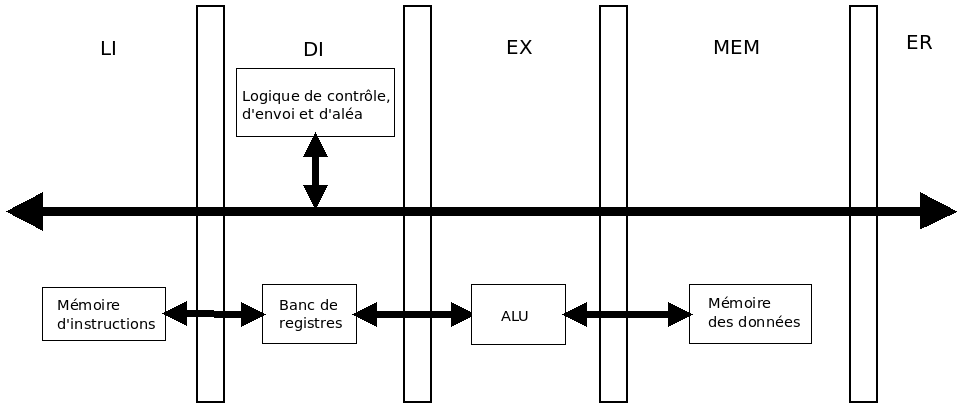
\includegraphics[scale=0.40]{archi-processeur.png}
    \caption{Architecture du processeur RISC}
    \label{archi-processeur}
\end{figure}

\subsubsection*{L'unité arithmétique et logique}

L'ALU effectue les opérations sur des mots de 8 bits. Les 4 bits de contrôle permettent de choisir l'opération à exécuter. Nous avons dû réfléchir à quel moment mettre à jour les flags qui serviront plus tard au saut conditionnel. À chaque opération, le flag \textbf{N} se met à jour en récupérant directement le bit de poids fort du résultat. Quant au flag \textbf{Z}, il passe à un si le résulat est égal à zéro. Le résultat de l'addition, la soustraction et la division tienne sur 8 bits sauf lorsqu'une retenue s'est propagée et celle-ci devient le flag \textbf{C}. Pour terminer, l'\textit{overflow} ne se produit que lorsqu'on a les cas énumérés dans le tableau ci-dessous (fig.\ref{tab:overflow-cases}). Lorsqu'on multiplie deux nombres de 8 bits, le résultat peut tenir sur 16 bits au maximum. Il faudra donc regarder pour le bit de signe le bit 15 alors que pour les autres opérations, ce sera le bit 7. De plus, lors d'une multiplication, tout dépassement au-delà de 8 bits doit être interprété comme un \textit{overflow} car le résultat renvoyé est sur 8 bits.

\begin{table}[h!]
  \centering
  \begin{tabular}{| l | c | c | c |}
    \hline
    Opération & Opérande A (bit 7) & Opérande B (bit 7) & Résultat (bit 7 pour $+$, $-$ et $/$) \\
    & & & et bit 15 pour $*$) \\ \hline
    addition & $\oplus$ & $\oplus$ & $\ominus$ \\ \hline
    addition & $\ominus$ & $\ominus$ & $\oplus$ \\ \hline
    soustraction & $\oplus$ & $\ominus$ & $\ominus$ \\ \hline
    soustraction & $\ominus$ & $\oplus$ & $\oplus$ \\ \hline
    multiplication & $\ominus$ & $\ominus$ & $\ominus$ \\ \hline
    multiplication & $\ominus$ & $\oplus$ & $\oplus$ \\ \hline
    multiplication & $\oplus$ & $\ominus$ & $\oplus$ \\ \hline
    multiplication & $\oplus$ & $\oplus$ & $\ominus$ \\ \hline
    division & $\ominus$ & $\ominus$ & $\ominus$ \\ \hline
    division & $\ominus$ & $\oplus$ & $\oplus$ \\ \hline
    division & $\oplus$ & $\ominus$ & $\oplus$ \\ \hline
    division & $\oplus$ & $\oplus$ & $\ominus$ \\ \hline
  \end{tabular}
  \caption{Énumération des cas d'\textit{overflow} pour les opérations arithmétiques}
  \label{tab:overflow-cases}
\end{table}

\subsubsection*{Le banc de registres}

Il s'agit d'un banc de registres à double port de lecture composé de registres de 8 bits avec accès en lecture et en écriture.

\subsubsection*{Les bancs de mémoire}

La ROM et la RAM ressemblent beaucoup au banc de registres. Nous y reviendrons plus tard pour parler de certaines difficultés dues à notre première implémentation de ces modules.

\subsubsection*{Le chemin de données}

Le chemin de données s'est constitué au fur et à mesure que l'on a intégré les modules. Reprenons le schéma de la figure \ref{archi-processeur} pour suivre le chemin d'une instruction et y voir plus clair. La première étape a consisté à créer les 4 regisres LI, DI, EX, MEM et ER. Il faut ensuite articuler toute la logique de contrôle autour de ces 4 registres.\\

Le premier étage consiste au chargement (\textit{fetch}) de l'instruction présente dans la ROM à l'adresse pointé par le PC (pointeur sur la prochaine instruction). Nous avons créé un registre accueillant la valeur du PC à part du banc de registre alors que l'idéal après recul, aurait été d'utiliser un registre particulier dans le banc et de le consacrer à contenir la valeur du PC. Il en aurait été de même si nous avions implémenté les instructions \texttt{PUSH} et \texttt{POP}, il aurait fallu un autre registre dans le banc pour garder le pointeur de sommet de pile. C'est à partir de cet étage qu'on va injecter les \texttt{NOP} lors d'un aléa.\\

Le deuxième étage va permettre de récupérer la valeur des registres opérandes si l'opération le nécessite. Il existe deux cas particuliers : l'instruction d'affichage \texttt{PRI} et les sauts \texttt{JMP} et \texttt{JMF}.\\
Le contenu du registre spécifié par \texttt{PRI} est chargé dans un registre interne au processeur que le  contrôleur de l'afficheur 7 segments va venir lire avec une fréquence de 1KHz pour ensuite aller afficher sa valeur en hexadécimal.\\
En ce qui concerne les sauts, on va aller récupérer la valeur du PC et la charger dans la partie C de l'instruction qui n'était jusqu'à présent pas utilisée. Cette valeur va être utilisée au niveau de l'ALU afin de calculer la nouvelle valeur du PC.\\
 
Le troisième étage consiste à récupérer le sortie de l'ALU et recupérer également la valeur des flags selon l'opération.\\

Le quatrième étage permet de stocker ou récupérer une valeur à une adresse de la RAM. Un multiplexeur asynchrone permet de choisir la bonne partie de l'opération à passer en adresse et en donnée à la RAM.\\

Le cinquième étage a pour charge d'affecter les registres. Il est composée lui aussi d'un multiplexeur et est très semblable au quatrième étage.

\section{Les points difficiles}
\subsection{Le chemin de données}

Au départ, tous les éléments (sauf l’ALU) étaient synchrones, tout comme chaque étage du pipeline. Plaçons nous par exemple au niveau du bloc de registres et du premier étage LI/DI (voir figure \ref{schema-lidi-registres}) :

\begin{figure}[!h]
    \centering
    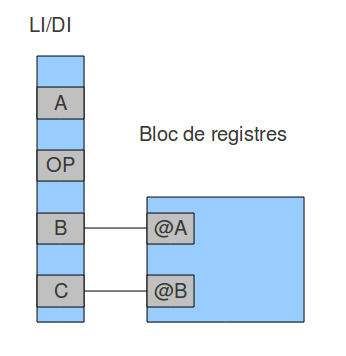
\includegraphics[scale=0.45]{schema-lidi-registres.png}
    \caption{Zoom sur le bloc de registres et le premier étage LI/DI du pipeline}
    \label{schema-lidi-registres}
\end{figure}

Lors d’un tick d'horloge, LI/DI met à jour ses sorties B et C. Le bloc de registres prend aussi en compte lors de ce tick la valeur de ses entrées @A et @B avec le B et C de LI/DI, sauf que ces dernières n’ont pas eu le temps de se mettre en jour quand les entrées @A et @B du bloc de registres capturent leur entrée. Du coup, il fallait un autre tick pour que le bloc de registre prenne en compte les bonnes valeurs. Cela décalait toute la propagation dans le pipeline. Nous avons donc tout mis en asynchrone pour ne laisser que les étages du pipeline calés sur la clock.

\subsection{La gestion des aléas}

La gestion des aléas est difficile, tous les prendre en compte est une tâche ardue. Le problème avec les aléas est de définir le lien entre chaque opération. Par exemple, prenons ces deux instructions : \texttt{COP R0 R1} suivit de \texttt{COP R2 R0}. Après avoir chargé les instructions dans le pipeline, la première instruction se trouve dans le registre DI/EX et la deuxième dans LI/DI. À cette étape-là, on a chargé les valeurs des registres \texttt{R0} et \texttt{R1} mais l'opération ne prendra effet sur les registres qu'après passage de l'étage MEM/ER. On voit bien dans ce cas que la prochaine opération, si on ne gère pas l'aléa, récupèrera la vieille valeur de \texttt{R0} qui était censée être écrasée à l'opération précédente. Il va falloir donc générer une bulle (injection de \texttt{NOP}) en attendant que l'instruction précédente ait affecté le registre \texttt{R0}. On peut trouver des aléas dans beaucoup de cas (opérations arithmétiques, saut, \ldots), c'est pourquoi il est difficile d'être exhaustif. Le plus sûr moyen de les éviter serait de créer des bulles à chaque opération mais alors le pipeline n'aurait plus aucun intérêt.\\

Notre processeur gère bien les aléas liés à chaque opération. On pouvait distinguer deux familles :
\begin{itemize}
\item{ceux liés aux registres}
\item{ceux liés aux sauts inconditionnels}
\item{ceux liés aux sauts conditionnels}
\end{itemize}

\vspace{10pt}

On a créé un contrôleur qui se base sur le contenu des quatres registres du pipeline et suivant leurs valeurs va activer une des trois sorties :
\begin{itemize}
\item{sortie \texttt{alea} : on surveille les numéros de registres situé à la partie A de l'instruction car c'est lui qui recevra le résultat de l'opération. Si dans les instructions suivantes, le numéro de registre situé en B ou C est le même, il va falloir attendre que l'opération  atteigne le dernier étage du pipeline pour être traitée. En attendant, on injecte des \texttt{NOP}.}

\item{sortie \texttt{jump\_JMP} : on injecte des \texttt{NOP} à la place des prochaines opérations et on propage notre \texttt{JMP} jusqu'à la sortie de l'ALU où on va récupérer la nouvelle valeur de l'IP (\textit{Instruction Pointer}) et lui affecter. Ce n'est qu'après affectation de cette valeur que l'on va pouvoir reprendre le \textit{fetch} des opérations.}

\item{sortie \texttt{jump\_JMF} : on injecte des \texttt{NOP} à la place des prochaines opérations et on propage notre \texttt{JMF} jusqu'à la sortie de l'ALU. La valeur du registre de condition récupérée à  l'étage DI/EX stocke le résultat de la condition booléenne. Suivant cette valeur (1 pour \texttt{true}, 0 pour \texttt{false}), soit on arrête d'injecter des \texttt{NOP} et on continue le cycle normal, soit on saute à l'adresse récupérée en sortie de l'ALU (cette adresse doit être calculée car le décalage est relatif donc nécessite un calcul par rapport à la position courante).}
\end{itemize}

\vspace{10pt}

Voici un extrait du code du contrôleur d'aléas :
\begin{lstlisting}[language=VHDL]
  --------------------------------------------------------------
  -- GESTION DES ALEAS
  --------------------------------------------------------------
  alea <= '1' when (	(
  -- gestion de la copie et du store
  (LIDI(INDEX_OP) = COP or LIDI(INDEX_OP) = STORE)
  and (
  (LIDI(INDEX_B) = DIEX(INDEX_A) and DIEX(INDEX_OP) /= NOP) or
  (LIDI(INDEX_B) = EXMem(INDEX_A) and EXMem(INDEX_OP) /= NOP))
  ) or (
  -- gestion des operations arithmetiques
  (LIDI(INDEX_OP) = ADD
  or LIDI(INDEX_OP) = MUL
  or LIDI(INDEX_OP) = DIV
  or LIDI(INDEX_OP) = SUB
  or LIDI(INDEX_OP) = INF 
  or LIDI(INDEX_OP) = SUP
  or LIDI(INDEX_OP) = EQU )
  and (
  (LIDI(INDEX_B) = DIEX(INDEX_A) and DIEX(INDEX_OP) /= NOP) or
  (LIDI(INDEX_B) = EXMem(INDEX_A) and EXMem(INDEX_OP) /= NOP) or
  (LIDI(INDEX_C) = DIEX(INDEX_A) and DIEX(INDEX_OP) /= NOP) or
  (LIDI(INDEX_C) = EXMem(INDEX_A) and EXMem(INDEX_OP) /= NOP)
  )
  )
  )
  else '0';
  
  jump_JMP <= '1' when ( (LIDI(INDEX_OP) = JMP and DIEX(INDEX_OP) /= NOP) or DIEX(INDEX_OP) = JMP or EXMem(INDEX_OP) = JMP )
  else '0';
  
  jump_JMF <= '1' when (LIDI(INDEX_OP) = JMF and DIEX(INDEX_OP) /= NOP) or DIEX(INDEX_OP) = JMF or EXMem(INDEX_OP) = JMF
  else '0';
\end{lstlisting}

Lorsqu'on a récupéré le résultat du contrôleur d'aléas et qu'une des trois sorties est activée, il faut d'abord décrémenter le PC. Ceci nous permet de retourner à l'adresse de l'instruction précédente pour pouvoir la recharger lorsque l'aléa sera terminé. On bloque ensuite l'incrémentation du PC jusqu'à disparition de l'aléa.

\section{Programmes de tests :}
Ce programmame de test est assez simple, il effectue un saut de 4 instructions (@4 $\rightarrow$ @9), puis fini par déborder du programme et tombe sur de la mémoire où il n'y a que des \texttt{NOP}.

\begin{lstlisting}[language=VHDL]
--extrait du code de ROM.vhd

registres(0) <= X"000C0200"; --AFC R0,0x02 --2
registres(1) <= X"010B0000"; --COP R1,R0 -- 2
registres(2) <= X"02010001"; --ADD R2, R0, R1 R2<-R0+R1 -- 4
registres(3) <= X"04020002"; --MUL R4, R0, R2 R4<-R0*R2 -- 8
registres(4) <= X"00050400"; --JMP 0x4 (ip <= ip +4)
-- portion sautee
registres(5) <= X"060C2300"; --AFC R6,0x23
registres(6) <= X"070C7800"; --AFC R7,0x78
registres(7) <= X"090C9900"; --AFC R9,0x99
registres(8) <= X"020E0400"; --STORE 0x2, R4
-- fin de la portion sautee
registres(9) <= X"040D0200"; --LOAD R4, 0x2 -- 0 (valeur par defaut dans la RAM)
registres(11) <= X"0D070100"; --INF R13, R1 , R0 => false
registres(12) <= X"0E070004"; --INF R14, R0 , R4 => false
registres(13) <= X"0F090100"; --EQU R15, R1 , R0 => true
registres(14) <= X"0C090400"; --EQU R12, R4 , R0 => false
registres(15) <= X"0B080400"; --SUP R11, R4 , R0 => false
registres(16) <= X"0A080004"; --SUP R10, R0 , R4 => true
registres(17) <= X"000A0000"; --PRI R0 -- affiche 2
registres(18) <= X"0006FA0F"; --JMF R15, 0xFA
                              --(jump -6 impossible car R15 = true)
registres(19) <= X"0006010D"; --JMF R13, 0x01 (jump +1 avec R13 = false)
\end{lstlisting}

Une portion du chronogramme de ce test est présentée en figure \ref{simulation}. Le chronogramme présente le moment où le \texttt{JMP} est en train d'être exécuté. On voit bien la bulle générée due à la détection de l'aléa \texttt{jump\_JMP} ainsi que le saut de IP (\textit{Instruction Pointer}) de \texttt{0x06} à \texttt{0x09}.

\newpage

\begin{figure}[!H]
    \centering
    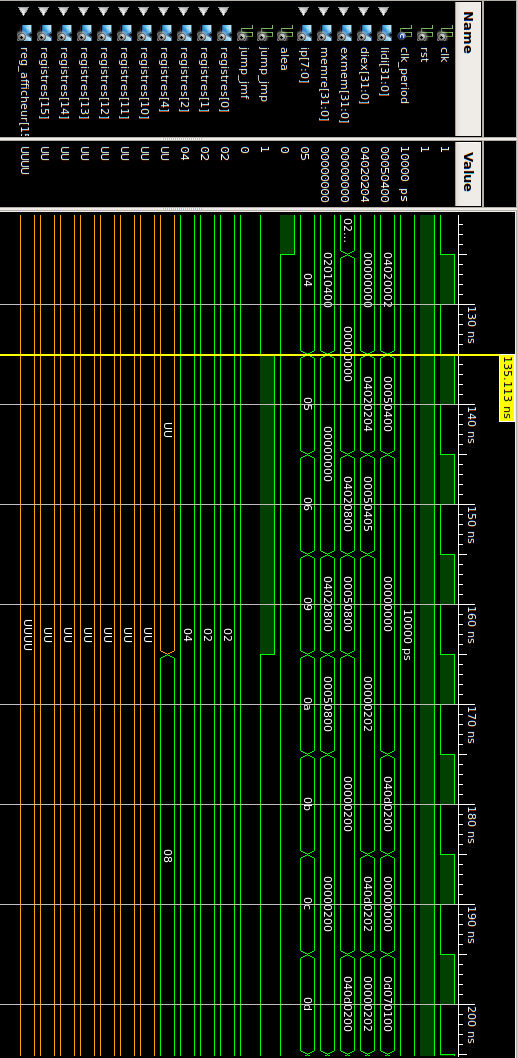
\includegraphics[scale=0.61]{simulation.png}
    \caption{Chronogramme de la simulation au moment du \texttt{JMP}}
    \label{simulation}
\end{figure}

\newpage

\section{Reste à faire et améliorations}
\subsubsection*{Partionnement en module}

Nous n'avons pas bien codé le chemin de données. Il aurait fallu créer des sous-modules comme pour le contrôleur des aléas. Cela aurait été plus facile à gérer et deboger.

\subsubsection*{Gestion complète des flags}

Nous ne gérons pas complètement les flags au niveau de l'ALU. Le flag d'\textit{overflow} ne marche que pour les additions. Le travail est déjà en partie fait puisqu'on a détaillé lors de la description de l'ALU les différents cas, il ne reste plus qu'à l'implémenter.

\subsubsection*{Implémentation de la division}

La division n'a pu être implémentée au niveau matériel car les bibliothèques fournies ne permettaient pas de directement effectuer une division. Il aurait fallu implémenter nous-même ce module mais par manque de temps, nous n'avons pas commencé. De plus, ce module n'est pas si simple que ça à implémenter. Dans un avenir immédiat, le plus rapide et le plus simple serait de gérer la division par 2 qui ne nécessite qu'un décalage à gauche. Ensuite en jouant avec les instructions en assembleur, une succession de décalages à gauche et de soustractions nous emmèneraient au résultat pour n'importe quelle division.

\newpage

\chapter{Développement du compilateur}

Le développement du compilateur s'est déroulé en deux phases.\\
Premièrement, nous avons réalisé un analyseur lexical qui détectait les mots de notre langage C. Puis une fois celui-ci opérationnel, nous avons développé l'analyseur syntaxique qui vérifiait que notre fichier C était bien formé.\\
Dans un deuxième temps, nous avons rajouté à l'analyseur syntaxique la génération d'un code intermédiaire qui plus tard allait être transformé en code binaire grâce au cross-compilateur.\\
Mais avant d'aller plus loin dans les explications, nous allons présenter le langage C supporté par notre compilateur.

\newpage

\section{Le langage C reconnu}
\subsection{La partie déclaration}

Le compilateur reconnaît toutes les formes de déclarations demandées, à savoir les variables entières constantes et non constantes. Il est possible de déclarer plusieurs variables à la suite séparées par des virgules. L’affectation est aussi possible au choix au niveau de la déclaration. Elle est par contre obligatoire pour les constantes.\\

Exemples de déclarations reconnues :
\begin{minted}[fontsize=\scriptsize]{c}
  int a;
  int toto, b = 31, c = 2e2, d = 1E1, e = -1;
  const int L = 10;
\end{minted}

\vspace{10pt}

Contrairement aux standards actuels C, il n’est pas possible de faire des déclarations autre part qu’au début de chaque bloc (début du \texttt{main}, des \texttt{if} ou des \texttt{while}).\\
La portée des variables est également implémentée. On peut utiliser une variable déclarée à une profondeur inférieure. On peut également déclarer une variable qui a le même identificateur qu’une déclarée à une profondeur inférieure.

\begin{minted}[fontsize=\scriptsize]{c}
  // profondeur 1
  int a;
  
  if (condition) {
    
    // profondeur 2
    int a;
    
    a = 1; // fait reference au 'a' declaree au-dessus
  }
\end{minted}

\subsection{Les opérations arithmétiques}

Il est possible d'utiliser les quatre opérations arithmétiques de base ($+$, $-$, $*$, $/$) sous forme parenthésée. On peut les placer où l'on veut (dans une affectation, une condition logique ou encore dans un \texttt{printf}).

\subsection{Les opérations logiques}

La gestion des booléens est la même qu’en C, l'entier 0 est interprété comme \textit{false} et tout le reste comme \textit{true}.\\
On peut réaliser des opérations logiques dans les parties conditions des \texttt{if} et des \texttt{while} mais aussi stocker l'évaluation d'une condition dans une variable.\\
Concernant les opérateurs logiques, \texttt{OR} (\texttt{||}), \texttt{AND} (\texttt{\&\&}) et \texttt{NOT} (\texttt{!}) sont utilisables. On peut comparer deux expressions arithmétiques avec \texttt{<}, \texttt{>}, \texttt{<=}, \texttt{>=}, \texttt{==} ou \texttt{!=}.\\

Exemples :
\begin{minted}[fontsize=\scriptsize]{c}
  /* fonctionnel */
  
  int a = a > 0;
  
  while ((a || 1 > 5)  && (b - (-8) + a >= 0)) {
    /* ... */
  }

  /* non implemente */
  while ( a = 1) {}
\end{minted}

\subsection{Les structures de contrôle}

\subsubsection*{Les alternatives}

Le \texttt{if} est similaire à celui du langage C avec un \texttt{if} suivi d’éventuellement d'un ou plusieurs \texttt{else if}, suivi(s) éventuellement d’un \texttt{else}. Les accolades sont obligatoires. On peut les imbriquer les unes dans les autres à souhait.

\subsubsection*{Les boucles}

Le \texttt{while} tout simple est implémenté avec accolades également obligatoires et imbrication.

\subsubsection*{Les fonctions}

Aucune fonction n'existe excepté le \texttt{printf} qui permet d’afficher sur la sortie standard la valeur d’un entier (à calculer ou non).\\
La seule fonction définissable est le \texttt{main}.

\section{Les composants du compilateur}
\begin{figure}[!h]
    \centering
    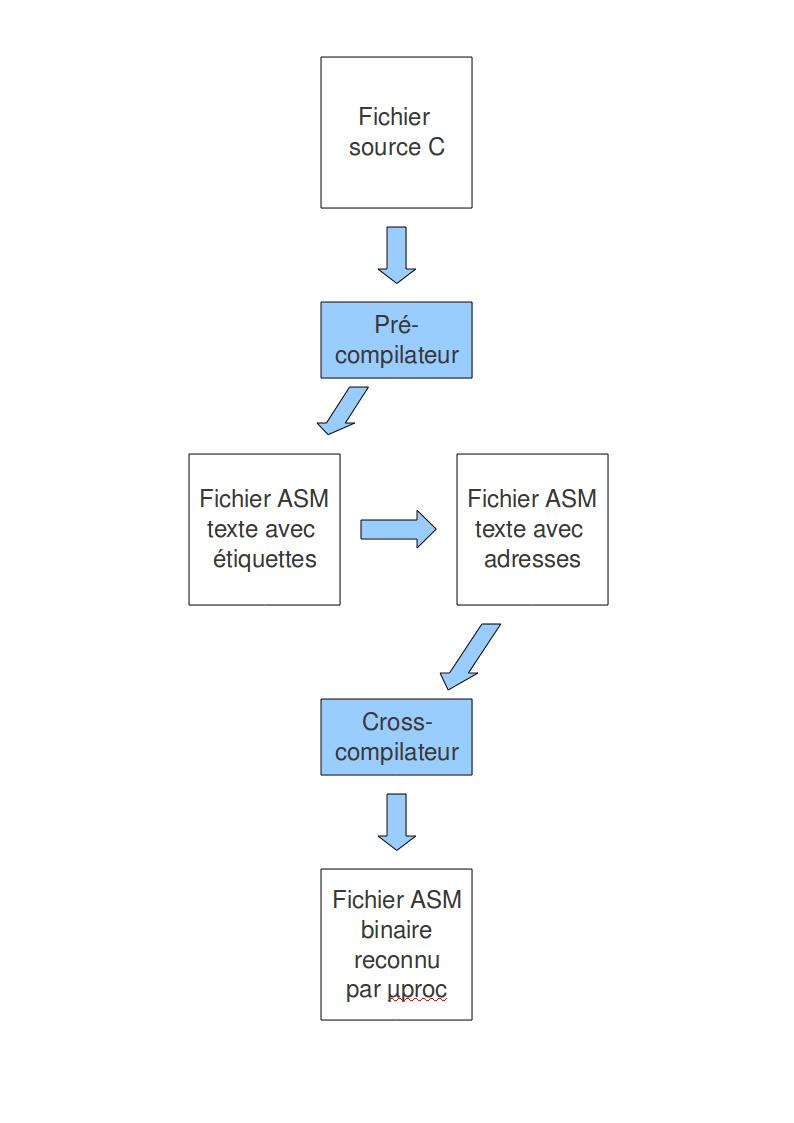
\includegraphics[scale=0.35]{global-compiler.jpg}
    \caption{Schéma de production du binaire exécutable depuis le code source C}
    \label{schema-compilation}
\end{figure}

\subsection{Le pré-compilateur}

\subsubsection{Sa fonction}

Le pré-compilateur a plusieurs fonctions. Tout d’abord, celui-ci fait l’analyse lexicale du fichier source C. Ensuite, l’analyse syntaxique vérifie toutes les règles grammaticales imposées par le langage présentées dans le partie précédente. Si une erreur est détectée, la compilation se poursuit jusqu’à la fin sans générer les fichiers assembleur pour montrer à l’utilisateur l’ensemble de ses erreurs.\\
L’assembleur intermédiaire est généré au fur et à mesure de l’analyse syntaxique. Les instructions prises en compte sont les mêmes que présentées dans le première partie à l'exception du \texttt{STORE} et du \texttt{LOAD} qui sont remplacés pour cette étape par un \texttt{COP}. Aucun registre n’est manipulé, on ne produit que des adresses correspondant à un emplacement dans une pile de valeurs.

\subsubsection{Gestion des variables et des valeurs intermédiaires}

Au stade du pré-compilateur, toutes les valeurs sont imaginées comme stockés dans une pile. Chaque variable ou valeur temporaire a donc une adresse.\\

Prenons l’exemple simple d’une affectation :
\begin{minted}[fontsize=\scriptsize]{c}
  a = a + 1;
\end{minted}

Pour évaluer l’expression de droite :
\begin{enumerate}
\item{Empiler la valeur de \texttt{a} au sommet de la pile}

\item{Empiler la valeur 1}

\item{Additionner les deux valeurs du sommet de pile}

\item{Affecter le résultat à la place du \texttt{a} temporaire}

\item{Mettre à jour la valeur de \texttt{a} avec celle temporaire}
\end{enumerate}

\vspace{10pt}

Pour gérer l’emplacement des variables dans la pile, on utilise la table des symboles. Sa structure est présentée dans la figure \ref{tab:structure-ligne}. Les variables sont insérées dans la table des symboles de la profondeur la plus haute à plus basse (c'est une pile de symboles). Ainsi, si on reprend l’exemple ci-dessous, pour récupérer l’adresse de la variable \texttt{a} de profondeur 2, on cherchera la première variable avec pour identifiant \texttt{a} en partant de la fin de la table des symboles.

\begin{minted}[fontsize=\scriptsize]{c}
  // profondeur 1
  int a = 0;
  
  if (condition) {
    // profondeur 2
    int a = 1;
    
    printf(a); // affiche 1
  }
\end{minted}

\begin{table}[h!]
  \begin{center}
  \begin{tabular}{| l | l | l | l | l |}
    \hline
    Identifiant & Profondeur & Constante & Initialisée & Adresse Pile\\
    \hline
  \end{tabular}
  \end{center}
  {\small
    \textit{Profondeur} permet de gérer la portée d’une variable et savoir si l’on peut déclarer telle variable à telle profondeur.\\
    \textit{Constante} permet de générer une erreur si l’on affecte une valeur à une constante.\\
    \textit{Initialisée} permet d’afficher un warning si la variable est utilisée sans avoir été initialisée.\\
  }
  \caption{Structure d'une ligne de la table des symboles}
  \label{tab:structure-ligne}
\end{table}

\subsubsection{Gestion des sauts}

La gestion des sauts se fait en deux étapes avec génération d'un fichier à la fin de chacune : le premier avec des étiquettes et le second avec des adresses.

\subsubsection*{Les sauts conditionnels}

Lorsqu'on produit le \texttt{JMF} on met une étiquette car on ne connaît pas le nombre d’instructions à sauter. Ce n’est qu’arrivé à la fin du bloc que l’on connaît cette adresse.\\
Pour gérer cela on utilise un tableau d’équivalence étiquette/adresse. À l’indice $n$ correspond l’adresse de l’étiquette \texttt{\$n}.\\
Les imbrications des structures de contrôle compliquent les choses. Il faut raisonner en LIFO : la première étiquette à déterminer est la dernière que l’on va trouver et la dernière étiquette à déterminer est la première que l’on va trouver. Autrement dit, à la fin d’un bloc de structure de contrôle, on remplit la première étiquette non-déterminée de la table en partant de la fin.\\

Voici un exemple de déroulement :
\begin{minted}[fontsize=\scriptsize]{c}
  if(/*...*/) {      //$0 => [ ]
    if(/*...*/){     //$1 => [ ; ]
      // instructions
    }                //$1 => [ ;@1]

    while(/*...*/) { //$2 => [ ; @1 ; ]
      // instructions
    }                //$2 => [ ; @1 ; @2]

    // instruction
  }                  //$0 => [@0 ; @1 ; @2]
\end{minted}

\subsubsection*{Les sauts inconditionnels}

Ils sont utilisés à la fin des blocs \texttt{if} contenant au moins un \texttt{else} après et permettent justement de ne pas aller dans le \texttt{else}, ou bien ils permettent de lancer l’itération suivante dans un \texttt{while}.\\
Pour les \texttt{if} il s’agit de faire un \texttt{JMP} à une étiquette commune. Au début d’un \texttt{if}, on empile dans une autre pile la valeur $i$  de cette étiquette, on consulte cette valeur à chaque fois que l’on insère un \texttt{JMP}. La pile permet là encore de permettre une imbrication de \texttt{if} \texttt{else if} les uns dans les autres. La valeur de l’étiquette est déterminée à la fin du \texttt{if} \texttt{else if}.\\

Voici un exemple de déroulement :
\begin{minted}[fontsize=\scriptsize]{c}
  if (/*...*/) {          // insertion $i : [$i]
    // instructions
    // JUMP $i
  } else if (/*...*/) {
    if (...) {            // insertion $m : [$i,$m]
      // JUMP $m
    } else {

    }
                          // $m : cible du JUMP => adresse $m determinee
                          // depile $m : [$i]
    // JUMP $i
  } else if (/*...*/) {
    // instructions
    // JUMP $i
  } else {
    // intruction
  }
                          // $i : cible des JUMP => adresse de $i determinee
\end{minted}

Pour les \texttt{while}, la technique est un peu différente puisqu’on connait dès le départ l’adresse de l’étiquette mais on ne sait pas où on va placer l’étiquette. On insère donc dans la table des étiquettes une nouvelle étiquette avec son adresse mais en négatif. Arrivé à la fin du \texttt{while}, on recherche la dernière adresse qui est négative et on retrouve l’étiquette associée. Il est ici inutile de mettre une étiquette, on pourrait mettre directement l’adresse puisqu’on la connaît. Mais, cela a été fait pour garder une certaine cohérence du fichier assembleur qui ne sera généré qu’avec des étiquettes.

\subsubsection*{Passage des étiquettes aux adresses :}

Pour finir, à la fin de l’analyse syntaxique on obtient ce fichier assembleur avec des étiquettes mais on connaît toutes les équivalences étiquettes/adresses. On reparse donc le fichier (avec la librairie C) toutes les étiquettes sont remplacées par les bonnes adresses.

\subsection{Le cross-compilateur}

Le cross-compilateur est beaucoup plus simple que le pré-compilateur car celui-ci lui a facilité pas mal le travail.\\

Voici un exemple de fichier qu'il récupère du pré-compilateur.
\begin{lstlisting}
- begin declarations -
- end declarations -
1:	AFC 0xff 1
2:	JMF 0xff 24
- begin declarations -
3:	AFC 0xff 2
4:	NOP
5:	AFC 0xfe 7
6:	NOP
- end declarations -
7:	COP 0xfd 0xff
8:	AFC 0xfc 2
9:	EQU 0xfd 0xfd 0xfc
10:	COP 0xfc 0xff
11:	COP 0xfb 0xfe
12:	AFC 0xfa 7
13:	EQU 0xfb 0xfb 0xfa
14:	AFC 0xfa 1
15:	SUB 0xfb 0xfa 0xfb
16:	MUL 0xfc 0xfc 0xfb
17:	ADD 0xfd 0xfd 0xfc
18:	JMF 0xfd 23
- begin declarations -
19:	AFC 0xfd 0
20:	NOP
- end declarations -
21:	COP 0xfc 0xfd
22:	PRI 0xfc
23:	JMP 1
\end{lstlisting}

Vous pouvez noter la présence de \texttt{NOP} entre les \textit{tokens} \texttt{- begin declarations -} et \texttt{- end declarations -}. Ces deux \textit{tokens} permettent d'interpréter correctement l'instruction \texttt{AFC} suivant le contexte. Si c'est une déclaration de variable, \texttt{AFC} est remplacé par un \texttt{AFC} et un \texttt{STORE}. Un \texttt{AFC} ailleurs reste un \texttt{AFC}. Quant au \texttt{NOP}, il est tout simplement éliminé des intructions. Celui-ci ne servait qu'à garder le décalage pour les sauts du côté du pre-compilateur et n'a plus aucune raison d'être du côté du cross-compilateur.

Le cross-compilateur a deux tâches importantes. La première consiste à distinguer des adresses de variables stockées dans la pile (donc en RAM) de celles correspondant à des registres. La seconde est de traduire les adresses de registres en un numéro de registre.\\
La distinction des adresses de variables dans la RAM est permise du fait de la présences des \textit{tokens} de la zone de déclarations. On sait que l'adresse spécifée au niveau de l'\texttt{AFC} correspond à une variable de la pile. Désormais cette adresse sera présente dans un tableau référençant toutes les adresses de variables en RAM ainsi que leur adresse réelle dans la RAM.\\
Une fois qu'on a fait cette distinction, on peut effectuer en priorité une recherche dans ce tableau pour vérifier si ce n'est pas une adresse dans la RAM. Si c'est le cas, celle-ci est remplacée par sa valeur réelle. Si ce n'est pas une adresse de la pile, il va falloir remplacer cette adresse par un numéro de registre. Un tableau va lui aussi garder la trace des adresses correspondant à un regitre et les registres utilisés. À partir de ces informations, nous allons pouvoir allouer des registres selon nos besoins et les désallouer quand leur contenu n'est plus nécessaire.

\subsection{Le simulateur}

Nous avons codé un simulateur qui lit le fichier binaire généré par le cross-compilateur et exécute les intructions comme le ferait le microprocesseur. Nous pouvons afficher le contenu des registres et de la RAM. Celui-ci nous a permis de debogger efficacement le binaire généré par le cross-compilateur en affinant notre recherche. Nous aurions dû le développer plus tôt car il n'était pas lié au développement du compilateur et nous aurait facilité le développement du cross-compilateur.

\section{Difficultés}
Pour l'élaboration du compilateur, nous avons rencontré principalement des difficultés du côté de la grammaire dans le pré-compileur. Elle était ambiguë et manquait d'exhaustivité. Il a fallu la corriger petit à petit au fur et à mesure que l'on implémentait des fonctionnalités.\\
Nous aurions dû plancher un peu plus longtemps sur la grammaire afin de nous éviter des peines inutiles.

\section{Reste à faire et améliorations}
\subsubsection*{Ajout des commentaires}

Nous aurions aimé implémenter les commentaires en utilisant les états associés à Lex. Cependant malgré l’aide apportée par les enseignants, nous n’avons pas réussi à les faire fonctionner. Il aurait fallu y passer un peu plus de temps, mais le nombre de séances dont nous disposions ne nous a pas suffit.

\subsubsection*{Amélioration de la gestion des registres dans le cross-compilateur}

Actuellement, lorsque tous les registres ont été alloués, le cross-compilateur renvoit une erreur à l'utilisateur lui indiquant qu'il n'a plus de registres disponibles. Il faudrait créer un système de sauvegarde et de restauration des registres qui semble plutôt complexe à mettre en place. Il faudrait garder une trace quelque part des registres sauvegardés avec quelques informations comme le numéro de registre où était présente cette valeur, la valeur à restaurer, et enfin il faudrait détecter le bon moment pour restaurer ce registre pour la cohérence. Tout cela implique le rajout d'instructions supplémentaires ce qui ne nous arrange pas vraiment car les valeurs des sauts ne seraient plus valides et à recalculer.

\newpage

\chapter*{Conclusion} \addcontentsline{toc}{chapter}{Conclusion}
Au final, ce projet nous a donné une vue globale mais aussi précise sur toutes les étapes qui vont d’un programme source en ASCII à son exécution au niveau matériel. Cela nous a également permis de relier entre eux bon nombres d’enseignements des années précédentes et donc d’éclaircir certaines zones d’ombres. Le projet semblait au départ très ambitieux et en même temps très motivant. Nous aurions aimé avoir plus de temps pour implémenter d’autres fonctionnalités manquantes du langage C ainsi que certaines instructions matérielles comme \texttt{POP}, \texttt{PUSH}, \texttt{AND}, \texttt{XOR}, \ldots{} qui nous auraient facilité la traduction du langage C vers la langage assembleur.

 
\newpage

\addcontentsline{toc}{chapter}{Table des figures}
\listoffigures

\newpage

\chapter*{Code source} \addcontentsline{toc}{chapter}{Code source}

L'ensemble des sources du projet est disponible sur le dépôt Git suivant :\\
\url{https://github.com/matlo607/insa_RISC-processor-fpga_C-compiler}

\end{document}
